\documentclass[a4paper,12pt]{article}

%%% Работа с русским языком % для pdfLatex
\usepackage{cmap}					% поиск в~PDF
\usepackage{mathtext} 				% русские буквы в~фомулах
\usepackage[T2A]{fontenc}			% кодировка
\usepackage[utf8]{inputenc}			% кодировка исходного текста
\usepackage[english,russian]{babel}	% локализация и переносы
\usepackage{indentfirst} 			% отступ 1 абзаца

%%% Работа с русским языком % для XeLatex
%\usepackage[english,russian]{babel}   %% загружает пакет многоязыковой вёрстки
%\usepackage{fontspec}      %% подготавливает загрузку шрифтов Open Type, True Type и др.
%\defaultfontfeatures{Ligatures={TeX},Renderer=Basic}  %% свойства шрифтов по умолчанию
%\setmainfont[Ligatures={TeX,Historic}]{Times New Roman} %% задаёт основной шрифт документа
%\setsansfont{Comic Sans MS}                    %% задаёт шрифт без засечек
%\setmonofont{Courier New}
%\usepackage{indentfirst}
%\frenchspacing

%%% Дополнительная работа с математикой
\usepackage{amsfonts,amssymb,amsthm,mathtools}
\usepackage{amsmath}
\usepackage{icomma} % "Умная" запятая: $0,2$~--- число, $0, 2$~--- перечисление
\usepackage{upgreek}

%%% Страница
\usepackage{extsizes} % Возможность сделать 14-й шрифт

%% Шрифты
\usepackage{euscript}	 % Шрифт Евклид
\usepackage{mathrsfs} % Красивый матшрифт

%% Свои команды
\DeclareMathOperator{\sgn}{\mathop{sgn}} % создание новой конанды \sgn (типо как \sin)
\usepackage{csquotes} % ещё одна штука для цитат
\newcommand{\pd}[2]{\ensuremath{\cfrac{\partial #1}{\partial #2}}} % частная производная
\newcommand{\abs}[1]{\ensuremath{\left|#1\right|}} % модуль
\renewcommand{\phi}{\ensuremath{\varphi}} % греческая фи
\newcommand{\pogk}[1]{\!\left(\cfrac{\sigma_{#1}}{#1}\right)^{\!\!\!2}\!}

% Ссылки
\usepackage{color} % подключить пакет color
% выбрать цвета
\definecolor{BlueGreen}{RGB}{49,152,255}
\definecolor{Violet}{RGB}{120,80,120}
% назначить цвета при подключении hyperref
\usepackage[unicode, colorlinks, urlcolor=blue, linkcolor=blue, pagecolor=blue, citecolor=blue]{hyperref} %синие ссылки
%\usepackage[unicode, colorlinks, urlcolor=black, linkcolor=black, pagecolor=black, citecolor=black]{hyperref} % для печати (отключить верхний!)
\mathtoolsset{showonlyrefs=true} % Показывать номера только у тех формул, на которые есть \eqref{} в~тексте.


%% Перенос знаков в~формулах (по Львовскому)
\newcommand*{\hm}[1]{#1\nobreak\discretionary{}
	{\hbox{$\mathsurround=0pt #1$}}{}}

%%% Работа с картинками
\usepackage{graphicx}  % Для вставки рисунков
\graphicspath{{images/}{images2/}}  % папки с картинками
\setlength\fboxsep{3pt} % Отступ рамки \fbox{} от рисунка
\setlength\fboxrule{1pt} % Толщина линий рамки \fbox{}
\usepackage{wrapfig} % Обтекание рисунков и таблиц текстом
\usepackage{multicol}

%%% Работа с таблицами
\usepackage{array,tabularx,tabulary,booktabs} % Дополнительная работа с таблицами
\usepackage{longtable}  % Длинные таблицы
\usepackage{multirow} % Слияние строк в~таблице
\usepackage{caption}
\captionsetup{labelsep=period, labelfont=bf}

%%% Оформление
\usepackage{indentfirst} % Красная строка
%\setlength{\parskip}{0.3cm} % отступы между абзацами

%%% Теоремы
\theoremstyle{plain} % Это стиль по умолчанию, его можно не переопределять.
\newtheorem{theorem}{Теорема}[section]
\newtheorem{proposition}[theorem]{Утверждение}

\theoremstyle{definition} % "Определение"
\newtheorem{definition}{Определение}[section]
\newtheorem{corollary}{Следствие}[theorem]
\newtheorem{problem}{Задача}[section]

\theoremstyle{remark} % "Примечание"
\newtheorem*{nonum}{Решение}
\newtheorem{zamech}{Замечание}[theorem]

%%% Правильные мат. символы для русского языка
\renewcommand{\epsilon}{\ensuremath{\varepsilon}}
\renewcommand{\phi}{\ensuremath{\varphi}}
\renewcommand{\kappa}{\ensuremath{\varkappa}}
\renewcommand{\le}{\ensuremath{\leqslant}}
\renewcommand{\leq}{\ensuremath{\leqslant}}
\renewcommand{\ge}{\ensuremath{\geqslant}}
\renewcommand{\geq}{\ensuremath{\geqslant}}
\renewcommand{\emptyset}{\varnothing}

%%% Название разделов
\usepackage{titlesec}
\titlelabel{\thetitle.\quad}


\title{Laba 1.4.4}
\author{Георгий Демьянов}
\date{November 2016}
\usepackage[left=1.27cm,right=1.27cm,top=1.27cm,bottom=2cm]{geometry}

\begin{document} 

\renewcommand{\figurename}{\textbf{Рис.}}		%Чтобы вместо figure под рисунками писал "рис"
\renewcommand{\tablename}{\textbf{Таблица}}		%Чтобы вместо table над таблицами писал Таблица

\begin{center}
	{\Large Предисловие}
\end{center}

В предисловии я хотел бы написать о некоторых подводных камнях, которые будут ожидать при выполнении лабы 1.4.4, и дать пару советов. Я крайне не советую вообще браться за эту лабу, а точнее даже отговариваю от ее выполнения. Я ее делал на довольно старой установке, в 2016 году, как вопрос по выбору на экзамен. Рядом стояла какая-то новая недоделанная установка, про неё ничего сказать не могу.

Итак, вот несколько моментов, почему эта лаба, эта установка является крайне капризной штукой:
\begin{enumerate}
	\item Время. Это самое главное в этой работе. На ваши конечные результаты будут влиять тысячные (!!!) доли секунд измеренных периодов колебаний. Т.к. вы будете делать по 10 колебаний маятников, значит время придётся измерять до сотых, причём очень точно. Систематической ошибкой в данном случае (в моем отчёте она не учитывается) является ваша реакция. В среднем она составляет 0.1~--~0.3 секунды (хотите проверьте свою на каком-нибудь сайте). Соответственно, разделив на 10, получим точность измерения до сотых. А влияют на результаты тысячные доли. Вот и думайте, нафиг оно надо.
	
	Мой совет: не пользуйтесь секундомерами на телефонах. Это крайне неудобно. Проще всего использовать секундомеры, которые есть в лабораториях, потому что вам не нужно будет смотреть, куда тыкать пальцем~--- кнопку вы будете чувствовать.
	\item Если вы видите, что на установке что-то криво, что-то неровно (расстояние неравные, маятники разных длин)~--- позовите своего преподавателя или ответственного за установки. Все должно быть очень ровно и точно.
	\item Измеряйте период, отсчитывая время от положения максимального отклонения маятника вопреки совету практикума. Думаю, это будет удобнее.
	\item Если при измерении периодов синфазных или встречных колебаний начинаются биения~--- все будет очень плохо. Переделывайте, старайтесь изначально отклонить маятники на один и тот же угол, чтобы избежать биений, когда они не нужны.
	\item Во время эксперимента сверяйте свои значения. Просто прикиньте приблизительно, фигня получается или нет. А то потом можно получить очень весёлые результаты.
	\item Советую измерять хотя бы по два периода биений, чтобы была хоть какая-то точность. Пусть у вас будет 3 результата, а не 4-5, но они будут хорошие.
	\item После выполнения постройте графики $T(M)$. Теоретически, должна получиться гипербола. Если у вас не гиперболическая зависимость, скорее всего получится плохо.
\end{enumerate}
Вот собственно и все. И мой последний совет: если вы ещё не сделали эту работу~--- не делайте. Есть много других более достойных и неплохих лаб, которые можно подготовить как вопрос по выбору.

\vspace{0.5cm}
\pagestyle{empty}
Что ж, вот, что получилось у меня.

По поводу вопросов/опечаток писать \href{https://vk.com/id37346992}{сюда}.
\newpage
\begin{titlepage}
\begin{center} 
 
\large Московский физико-технический институт\\
Факультет молекулярной и химической физики\\
\vspace{32ex}
\huge Лабораторная работа №1.4.4\\
\textbf{\Large <<Исследование свободных колебаний
связанных маятников>>}\\
\end{center} 

\vspace{40ex}
{\par \raggedleft \large \emph{Выполнил:}\\ студент 1 курса\\ 642 группы ФМХФ\\ Демьянов Георгий\\ Сергеевич \par}
\begin{center}
\vfill Москва 2016
\end{center}
\end{titlepage}

\newpage
\pagestyle{plain}
\setcounter{page}{2}

\textbf{\emph{Цель работы:}} изучение колебательной системы с двумя степенями
свободы.

\textbf{\emph{Оборудование:}} установка с двумя одинаковыми математическими маятниками, бифилярно подвешенными на натянутую
горизонтально струну, секундомер, измерительная линейка.
\begin{center}
\vspace{0.5cm}{\parbox{16cm}{\small{\textbf{\centering{Аннотация}\\
				\hspace{0.6cm} В работе использовалась установка со связанными маятниками. С помощью линейки измерили длину маятников, расстояние между неподвижными точками струны и точками подвеса маятников. Далее секундомером измерили период синфазных и встречных колебаний. Также измерили период колебаний биений. Данный эксперимент повторили с несколькими грузами разных масс, которые натягивают нить, соединяющую маятники. С помощью полученных данных проверили соотношения, полученные теоретически.}}}}
\end{center}
\textbf{\section{Теоретическое введение}}
Измерения производятся на установке, изображённой на рис. \ref{ust}. На рис. \ref{ris2} показаны смещения точек C и D струны и отклонения маятников в вертикальной (рис. \ref{ris2}а) и горизонтальной (рис. \ref{ris2}б) плоскостях.

При небольших отклонениях маятников для силы натяжения подвеса маятника $T$ имеем (рис. \ref{ris2}а):
\begin{equation}
mg \approx T.
\label{1}
\end{equation}
Для движения маятников в горизонтальном направлении (рис. \ref{ris2}):
\begin{equation}
m\ddot{x}{_1} = -T\sin\varphi_1 \approx -T\cfrac{x_1-x_3}{l} \approx -mg\cfrac{x_1-x_3}{l},
\label{2}
\end{equation}
\begin{equation}
m\ddot{x}{_2} = -T\sin\varphi_2 \approx -T\cfrac{x_2-x_4}{l} \approx -mg\cfrac{x_2-x_4}{l}.
\label{3}
\end{equation}
Связь между натяжением струны и натяжением подвеса получаем
из рис. \ref{ris2}:
\begin{equation}
T\cfrac{x_1-x_3}{l}=F\cfrac{x_3}{a}+F\cfrac{x_3-x_4}{a},
\label{4}
\end{equation}
\begin{equation}
T\cfrac{x_2-x_4}{l}=F\cfrac{x_4}{a}+F\cfrac{x_4-x_3}{a}.
\label{5}
\end{equation}
Введем безразмерный параметр $\sigma$:
$$\sigma = \cfrac{T}{F}\cfrac{a}{l}=\cfrac{m}{M}\cfrac{a}{l},$$
который в нашем случае много меньше единицы (т.к. $m \ll M$). Тогда из \eqref{4} и \eqref{5} получаем 
\begin{equation}
\sigma x_1=(2+\sigma)x_3-x_4,\hspace{1cm}\sigma x_2=(2+\sigma)x_4-x_3.
\label{6}
\end{equation}
Т.к. $\sigma \ll 1$:
\begin{equation}
x_3=\sigma\cfrac{2x_1+x_2}{3},\hspace{1cm} x_4=\sigma\cfrac{x_1+2x_2}{3}.
\label{7}
\end{equation}
\begin{figure}
	\noindent\centering{
	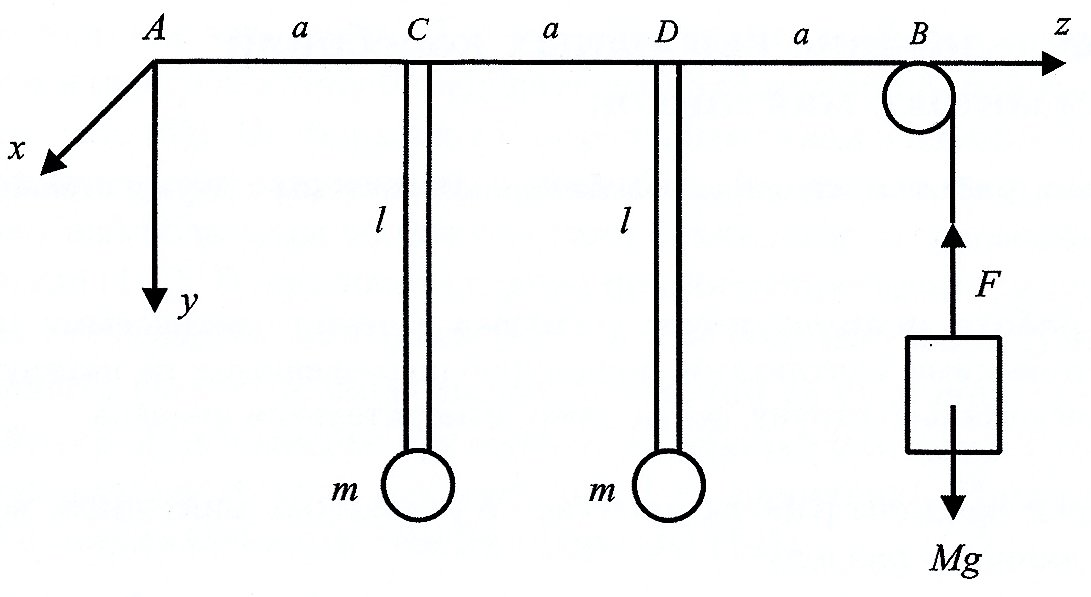
\includegraphics[width=17cm]{ust.jpg}
	}
	\caption{Общий вид установки}
	\label{ust}
	\vspace{0.5cm}
	\begin{minipage}[h]{0.45\linewidth}
		\centering{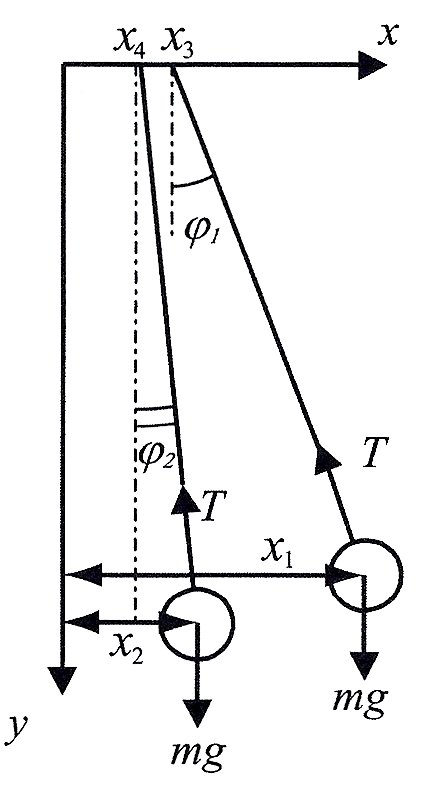
\includegraphics[width=7cm]{ust_a.jpg}} \\а) вид сбоку
	\end{minipage}
	\hfill
	\begin{minipage}[h]{0.45\linewidth}
		\centering{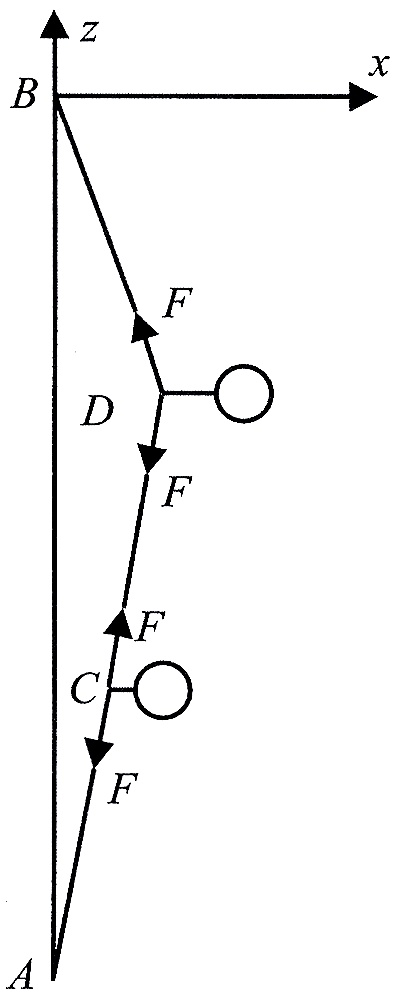
\includegraphics[width=5cm]{ust_b.jpg}} \\б) вид сверху
	\end{minipage}
	\hfill
	\caption{Отклонения маятников и струны}
	\label{ris2}
\end{figure}
Уравнения движения маятников примут вид:
\begin{equation}
\ddot{x}_1+\cfrac{g}{l} (1-\sigma)x_1=\sigma\cfrac{g}{3l}(x_2-x_1),
\label{8}
\end{equation}
\begin{equation}
\ddot{x}_2+\cfrac{g}{l} (1-\sigma)x_2=\sigma\cfrac{g}{3l}(x_1-x_2).
\label{9}
\end{equation}
Введем обозначения:
$$\cfrac{g}{l}(1-\sigma)=\omega^{\!\!2}_0, \hspace{1cm} \sigma\cfrac{g}{3l}=\omega^{\!\!2}_0 \varepsilon.$$
Разделив правое выражение на левое и домножив на 3, легко получить, что:
$$\cfrac{\sigma}{1-\sigma}=3\varepsilon \xrightarrow{\sigma \ll 1} \sigma(1+\sigma) \approx 3\varepsilon \xrightarrow{\sigma \ll 1} \sigma \approx 3\varepsilon.$$
Параметр $\varepsilon$ характеризует связь маятников. Тогда система уравнений \eqref{8}, \eqref{9} имеет вид:
\begin{equation}
\ddot{x}_1+\omega^2_0 x_1=-\omega^2_0\varepsilon(x_1-x_2),
\label{10}
\end{equation}
\begin{equation}
\ddot{x}_2+\omega^2_0 x_2=\omega^2_0\varepsilon(x_1-x_2).
\label{11}
\end{equation}
Сложим и вычтем:
\begin{equation}
(\ddot{x}_1+\ddot{x}_2)+\omega^2_0(x_1+x_2)=0,
\label{12}
\end{equation}
\begin{equation}
(\ddot{x}_1-\ddot{x}_2)+\omega^2_0(1+2\varepsilon)(x_1-x_2)=0.
\label{13}
\end{equation}

Таким образом, мы получили уравнения колебательного движения. Решения \eqref{12} и \eqref{13} имеют вид:
\begin{equation}
x_1+x_2=A\cos(\omega^{+}t+x'),
\label{14}
\end{equation}
\begin{equation}
x_1-x_2=B\cos(\omega^{-}t+x''),
\label{15}
\end{equation}
где $\omega^+=\omega_0$ и $\omega^-=\omega_0\sqrt{(1+2\varepsilon)}$, $A, B, x', x''$~--- произвольные константы. Сложим и вычтем \eqref{14} и \eqref{15}. Тогда получим зависимость $x_1(t)$ и $x_2(t)$:
\begin{equation}
x_1=\cfrac{1}{2}A\cos(\omega^{+}t+x')+\cfrac{1}{2}B\cos(\omega^{-}t+x''),
\label{16}
\end{equation}
\begin{equation}
x_2=\cfrac{1}{2}A\cos(\omega^{+}t+x')-\cfrac{1}{2}B\cos(\omega^{-}t+x'').
\label{17}
\end{equation}
Дифференцируя, найдём выражения для скоростей маятников:
\begin{equation}
\dot{x}_1=-\cfrac{1}{2}\,\omega^{+}A\sin(\omega^{+}t+x')-\cfrac{1}{2}\,\omega^{-}B\sin(\omega^{-}t+x''),
\label{18}
\end{equation}
\begin{equation}
\dot{x}_2=-\cfrac{1}{2}\,\omega^{+}A\sin(\omega^{+}t+x')+\cfrac{1}{2}\,\omega^{-}B\sin(\omega^{-}t+x'').
\label{19}
\end{equation}

Проанализируем полученные решения. Пусть маятники имеют вначале (при $t = 0$) одинаковые отклонения и нулевые начальные скорости:
$$x_1(0)=x_2(0)=x_0, \hspace{1cm} \dot{x}_1(0)=\dot{x}_2(0)=0.$$
Тогда из \eqref{16}, \eqref{17}, \eqref{18}, \eqref{19} находим:
$$\sin x'=0, \hspace{1cm} A=2x_0,\hspace{1cm} B=0,$$
т.е.
\begin{equation}
x_1=x_0\cos\omega^+t, \hspace{1cm} x_2=x_0\cos\omega^+t.
\label{20}
\end{equation}
Это означает, что маятники будут колебаться с одинаковой амплитудой и в одинаковой фазе (синфазно).

Если при $t = 0$
$$ x_1(0)=-x_2(0)=x_0, \hspace{1cm} \dot{x}_1(0)=\dot{x}_2(0)=0,$$
то из \eqref{16}~---~\eqref{19} следует:
$$\sin x''=0, \hspace{1cm} A=0, \hspace{1cm} B=2x_0,$$
т.е.
\begin{equation}
x_1=x_0\cos\omega^-t, \hspace{1cm} x_2=-x_0\cos\omega^-t=x_0\cos(\omega^-t+\pi).
\label{21}
\end{equation}
Соотношения показывают, что маятники колеблются с постоянной амплитудой, синхронно, но не синфазно: колебания маятников находятся
в противофазе. Два вида движения \eqref{20} и \eqref{21} называются \textbf{нормальными модами} колебаний системы связанных осцилляторов. Нормальная мода колебаний - это коллективное колебание, при котором
амплитуда колебаний каждой частицы остается постоянной.

Рассмотрим теперь случай, когда в начальный момент времени отклонен лишь один маятник, т. е.
$$x_1(0)=x_0, \hspace{1cm} x_2(0)=0, \hspace{1cm} \dot{x}_1(0)=\dot{x}_2(0)=0.$$
Тогда в этом случае:
\begin{equation}
x_1=\cfrac{x_0}{2}(\cos\omega^+t+\cos\omega^-t),
\label{22}
\end{equation}
\begin{equation}
x_2=\cfrac{x_0}{2}(\cos\omega^+t-\cos\omega^-t).
\label{23}
\end{equation}
Используя тригонометрические преобразования, представим \eqref{22} и \eqref{23} в виде:
\begin{equation}
x_1=x_0\cos\cfrac{\omega^+-\omega^-}{2}\,t\cdot\cos\cfrac{\omega^++\omega^-}{2}\,t,
\label{24}
\end{equation}
\begin{equation}
x_2=x_0\sin\cfrac{\omega^--\omega^+}{2}\,t\cdot\sin\cfrac{\omega^++\omega^-}{2}\,t.
\label{25}
\end{equation}

Проанализируем формулы \eqref{24} и \eqref{25}. $\omega^+=\omega_0$, где $\omega_0$~---~собственная частота одиночного маятника (\textbf{парциальная частота}), $\omega^-=\omega_0\sqrt{1+2\varepsilon},\, \varepsilon=\frac{1}{3}\sigma \ll 1.$ Тогда можно считать, что
$$\omega^-\approx\omega_0(1+\varepsilon),$$
т.е.
$$\omega^--\omega^+ \approx \omega_0\varepsilon, \hspace{1cm} \omega^-+\omega^+\approx2\omega_0.$$
Тогда уравнения \eqref{24}, \eqref{25} можно при этом представить приближенно в
виде
\begin{equation}
x_1=x_0\cos\cfrac{\omega_0\varepsilon}{2}\,t\cdot\cos\omega_0\,t,
\label{26}
\end{equation}
\begin{equation}
x_2=x_0\sin\cfrac{\omega_0\varepsilon}{2}\,t\cdot\sin\omega_0\,t=x_0\sin\cfrac{\omega_0\epsilon}{2}\,t\cdot\cos\left(\omega_0\,t-\cfrac{\pi}{2}\right).
\label{27}
\end{equation}

Таким образом, мы имеем дело с гармоническими колебаниями частоты $\omega_0$, амплитуда которых изменяется со временем периодически с гораздо меньшей частотой $\frac{1}{2}\omega_0\varepsilon$. Это~---~так называемые \textbf{амплитудномодулированные колебания}, или, другими словами, \textbf{биения}. Относительная фаза колебаний равна $\frac{\pi}{2}$. Модулированная амплитуда колебаний
первого маятника есть величина
\begin{equation}
A_1(t)=x_0\cos\cfrac{\omega_0\varepsilon}{2}\,t.
\label{28}
\end{equation}
Аналогично амплитуда колебаний второго маятника равна
\begin{equation}
A_2(t)=x_0\sin\cfrac{\omega_0\varepsilon}{2}\,t=x_0\cos\left(\cfrac{\omega_0\varepsilon}{2}\,t-\cfrac{\pi}{2}\right).
\label{29}
\end{equation}
В начальный момент времени $t=0$ имеем
$$A_1=x_0, \hspace{1cm} A_2=0.$$
В момент времени $t=\cfrac{\pi}{\omega_0\varepsilon}$
$$A_1=0, \hspace{1cm} A_2=x_0.$$
В момент времени $t=\cfrac{2\pi}{\omega_0\varepsilon}$
$$A_1=-x_0, \hspace{1cm} A_2=0.$$
Отметим, что амплитуда гармонического колебания, по определению,
величина положительная. Отрицательный знак здесь означает, что относительная фаза колебаний изменилась на $\pi$.\\ В момент времени $t=\cfrac{3\pi}{\omega_0\varepsilon}$
$$A_1=0, \hspace{1cm} A_2=-x_0.$$
В момент времени $t=\cfrac{4\pi}{\omega_0\varepsilon}$
$$A_1=x_0, \hspace{1cm} A_2=0.$$
Таким образом, происходит передача колебаний от одного маятника к другому (рис. \ref{bien}). 
\begin{center}
	\begin{figure}[h]
		\begin{minipage}{0.5\linewidth}
			\noindent\centering{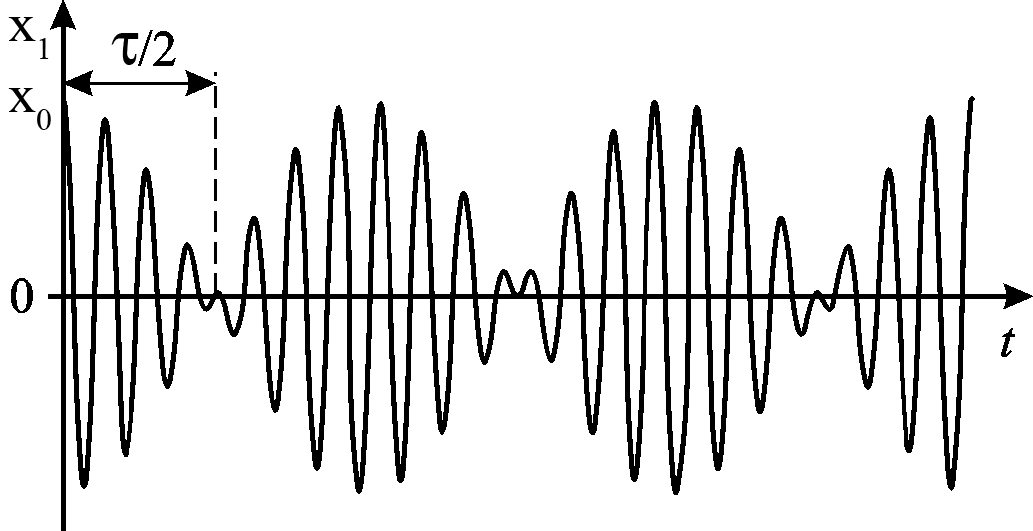
\includegraphics[width=9cm]{A9R1091.jpg}}\\ а) $x_1(t)$
		\end{minipage}
		\hfill
		\begin{minipage}{0.5\linewidth}
			\noindent\centering{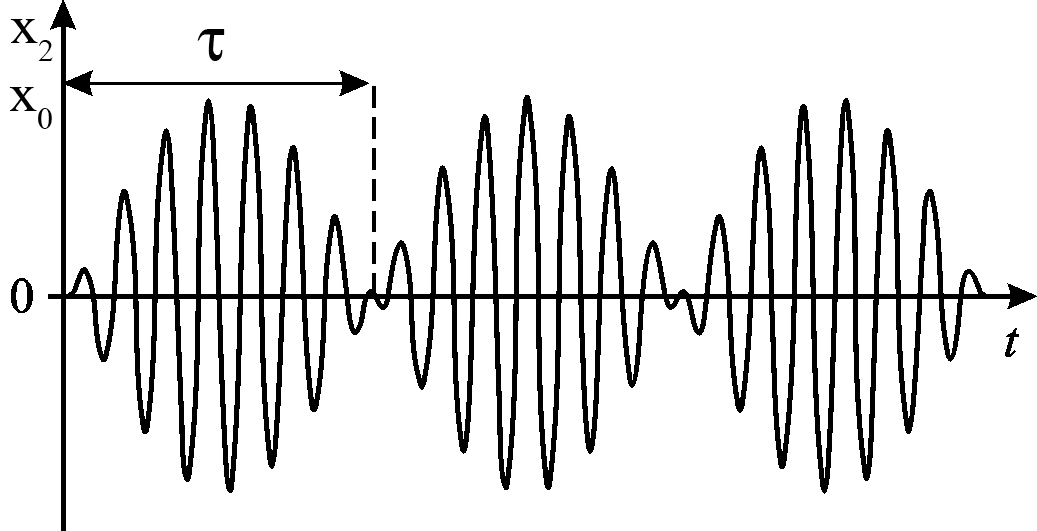
\includegraphics[width=9cm]{A9R109F.jpg}}\\ б) $x_2(t)$
		\end{minipage}
		\hfill
		\caption{Биения в системе двух идентичных
			связанных маятников}
		\label{bien}
		\vspace{-0.5cm}
	\end{figure}
\end{center}
Маятники обмениваются энергией. При $t=0$ вся энергия
сосредоточена в первом маятнике. В результате связи через пружину
энергия постепенно передается от первого маятника ко второму до тех
пор, пока в нем не накопится вся энергия. Время $\tau$, необходимое для
перехода энергии от одного маятника к другому и обратно, можно оценить из уравнения
$$\cfrac{\omega_0\varepsilon}{2}\,\tau=\pi,$$
т.е.
\begin{equation}
\tau=\cfrac{2\pi}{\omega_0\varepsilon},
\label{30}
\end{equation}
Частота, с которой осцилляторы обмениваются энергией, равна
\begin{equation}
\cfrac{2\pi}{\tau}=\omega_0\varepsilon=\omega^--\omega^+ \Rightarrow \cfrac{1}{\tau}=\cfrac{1}{T_2}-\cfrac{1}{T_1},
\label{31}
\end{equation}
где $$T_2=\cfrac{2\pi}{\omega^-},\qquad T_1=\cfrac{2\pi}{\omega^+}.$$
\vspace{5pt}Можно видеть, что параметр связи равен
\begin{equation}
\varepsilon=\cfrac{1}{3}\left(1-\cfrac{\omega^2_0l}{g}\right).
\label{32}
\end{equation}
В силу \eqref{32} соотношения \eqref{30} приобретает вид
\begin{equation}
\tau=\cfrac{6\pi}{\omega_0\left(1-\frac{\omega^2_0l}{g}\right)} \approx 6\pi\cfrac{Ml}{ma}\sqrt{\cfrac{l}{g}\,}.
\label{33}
\end{equation}

Формулы \eqref{31} и \eqref{33} можно проверить экспериментально, измеряя парциальную частоту маятника, его длину и время обмена энергией.

Теоретические выкладки и рисунки взяты из \cite{Gladun:PrakMech}~---~c. 229~--~233, 265~--~269.
\textbf{\section{Экспериментальная установка}}

Используемая установка изображена на рис. 1. Один конец струны прикреплён к вертикальной стойке установки,
а другой конец переброшен через неподвижный блок и натянут с помощью груза массой $M$. Точки струны A и B неподвижны. В точках
С и D, которые делят расстояние между A и B на три равные части
(каждая длиной $a$), подвешены одинаковые математические маятники
массой $m$ и длиной $l$. Каждый маятник подвешен на двух нитях в плоскости струны (бифилярно), чтобы колебания маятников происходили
в плоскостях, перпендикулярных струне. Сила натяжения струны намного больше веса маятников ($M \gg m$). Вертикальная составляющая
смещения струны никак не сказывается на движении маятников при
малых отклонениях. Горизонтальная составляющая смещения струны,
хотя она и мала по сравнению со смещениями маятников, осуществляет слабую связь между маятниками.

Описание установки взято из \cite{Gladun:PrakMech}~---~c. 265.

\textbf{\section{Обработка результатов}}

Измерим длину математического маятника $l$, расстояние между точками C и D равное $a$, массу шарика $m$. Получим следующие значения:
$$ l=(0.420 \pm 0.005)\  \text{м}, \qquad a=(0.262 \pm 0.005)\  \text{м}, \qquad m=(0.2270 \pm 0.0005)\  \text{кг}.$$

Далее будем измерять время $N=10$ синфазных ($t_1$), встречных ($t_2$) и парциальных ($t_0$) колебаний, а также измерим время биений $\tau$ при разной массе $M$ грузов, которые натягивают струну. Полученные данные занесём в таблицу\footnote{Точность масс грузов слишком большая, советую оставить 3 знака после запятой и погрешность $\pm 0.001$ кг. Так будет ближе к правде.} \ref{my-label}.
\begin{table}[h!]
	\centering
	\caption{Полученные значения}
	\label{my-label}
	\begin{tabular}{|c|c|c|c|c|}
		\hline
		$M$, кг                               & $\tau_{\text{экс}}$, с              & $t_1$, с & $t_2$, с & $t_0$, с \\ \hline
		\multirow{3}{*}{1.89510 $\pm$ 0.00005} & \multirow{3}{*}{53.07} & 13.59    & 13.25    & 13.47    \\ \cline{3-5} 
		&                        & 13.60    & 13.24    & 13.48    \\ \cline{3-5} 
		&                        & 13.59    & 13.29    & 13.49    \\ \hline
		\multirow{3}{*}{2.91060 $\pm$ 0.00005} & \multirow{3}{*}{69.02} & 13.48    & 13.21    & 13.43    \\ \cline{3-5} 
		&                        & 13.48    & 13.26    & 13.40    \\ \cline{3-5} 
		&                        & 13.48    & 13.24    & 13.44    \\ \hline
		\multirow{3}{*}{3.72580 $\pm$ 0.00005} & \multirow{3}{*}{80.65} & 13.44    & 13.27    & 13.32    \\ \cline{3-5} 
		&                        & 13.45    & 13.26    & 13.33    \\ \cline{3-5} 
		&                        & 13.49    & 13.25    & 13.34    \\ \hline
		\multirow{3}{*}{4.47510 $\pm$ 0.00005} & \multirow{3}{*}{90.41} & 13.34    & 13.16    & 13.31    \\ \cline{3-5} 
		&                        & 13.37    & 13.18    & 13.30    \\ \cline{3-5} 
		&                        & 13.35    & 13.15    & 13.27    \\ \hline
		\multirow{3}{*}{5.29730 $\pm$ 0.00005} & \multirow{3}{*}{98.34} & 13.32    & 13.18    & 13.28    \\ \cline{3-5} 
		&                        & 13.33    & 13.14    & 13.29    \\ \cline{3-5} 
		&                        & 13.34    & 13.16    & 13.24    \\ \hline
	\end{tabular}
\end{table}
Далее найдём периоды колебаний, разделив время колебаний на 10 и найдя их среднее значение
$$T_i=\bar{T}_i, \hspace{1cm} i=0, 1, 2.$$
Также найдём погрешность измерений $T_1, T_2, T_0$ по формуле
\begin{equation}
\sigma_{T_i}=\sqrt{\cfrac{1}{3-1}\sum_{k=1}^3 \left(T_k-\bar{T}_i\right)^{\!2}}, \hspace{1cm} i=0, 1, 2.
\label{34}
\end{equation}
Полученные значения внесём в таблицу \ref{my-label1}.
\begin{table}[h!]
	\centering
	\caption{Полученные значения}
	\label{my-label1}
	\begin{tabular}{|c|c|c|c|c|c|c|}
		\hline
		$M$, кг               & $T_1$, с & $\sigma_{T_1}$, с & $T_2$, с & $\sigma_{T_2}$, с & $T_0$, с & $\sigma_{T_0}$, с \\ \hline
		1.89510 $\pm$ 0.00005 & 1.3593   & 0.0006            & 1.326    & 0.003             & 1.3480   & 0.0010             \\ \hline
		2.91060 $\pm$ 0.00005  & 1.348    & 0.000                 & 1.324    & 0.003             & 1.342    & 0.002              \\ \hline
		3.72580 $\pm$ 0.00005  & 1.346    & 0.003             & 1.326    & 0.001             & 1.3330   & 0.0010             \\ \hline
		4.47510 $\pm$ 0.00005 & 1.3353   & 0.0015            & 1.3163   & 0.0015            & 1.329    & 0.002              \\ \hline
		5.29730 $\pm$ 0.00005 & 1.333    & 0.001             & 1.316    & 0.002             & 1.327    & 0.003              \\ \hline
	\end{tabular}
\end{table}

\subsection{Проверка уравнения (\ref{31})}
Проверим соотношение \eqref{31}, полученное теоретически. Для этого найдём по формуле \eqref{31} $\tau=\cfrac{1}{\frac{1}{T_2}-\frac{1}{T_1}}$. Погрешность $\tau$ определим так:
\begin{equation}
\sigma^2_{\tau}=\left(\cfrac{\partial\tau}{\partial T_1}\right)^{\!2}\!\sigma^2_{T_1}+\left(\cfrac{\partial\tau}{\partial T_2}\right)^{\!2}\!\sigma^2_{T_2},
\label{35}
\end{equation}
где
$$\cfrac{\partial\tau}{\partial T_1} = -\cfrac{T^2_1}{\left(T_1-T_2\right)^2}$$
$$\cfrac{\partial\tau}{\partial T_2} = \cfrac{T^2_2}{\left(T_1-T_2\right)^2}$$
Тогда подставив все значения, занесём полученные данные в таблицу \ref{my-label_31} соответственно массам по возрастанию.
\begin{table}[h!]
	\centering
	\caption{$\tau$, рассчитанное по \eqref{31}}
	\label{my-label_31}
	\begin{tabular}{|c|c|}
		\hline
		$\tau$, с & $\sigma_{\tau}$, с \\ \hline
		54        & 4                  \\ \hline
		73        & 7                  \\ \hline
		89        & 13                 \\ \hline
		93        & 11                 \\ \hline
		103       & 13                 \\ \hline
	\end{tabular}
\end{table}

Таким образом, мы видим, что значения, полученные из соотношения \eqref{31}, совпали с экспериментальными в пределах погрешности. Заметим, что значения погрешностей получились достаточно велики. Это объясняется тем, что периоды $T_1$ и $T_2$ близки друг к другу, и разность $T_1-T_2$, находящаяся в знаменателе выражения для погрешности, получается очень маленькой.

\subsection{Проверка уравнения (\ref{33})}
Теперь проверим соотношение \eqref{33}. Сначала проверим точное равенство (через $\omega_0$, которое найдём, зная период парциальных колебаний), а после проверим приближенное равенство.

\subsubsection{Проверка точного равенства}
Рассчитаем $\omega_0$ для каждого значения $T_0$ по известной формуле:
$$ \omega_0=\cfrac{2\pi}{T_0},$$
и погрешность
$$\cfrac{\sigma_{\omega_0}}{\omega_0}=\cfrac{\sigma_{T_0}}{T_0}.$$
Подставив значения, занесём данные в таблицу \ref{my-label3} (снова по возрастанию значений масс грузов).
\begin{table}[h!]
	\centering
	\caption{Значения $\omega_0$}
	\label{my-label3}
	\begin{tabular}{|c|c|}
		\hline
		$\omega_0$, с$^{-1}$ & $\sigma_{\omega_0}$, с$^{-1}$ \\ \hline
		4.661                & 0.003                         \\ \hline
		4.681                & 0.007                         \\ \hline
		4.714                & 0.004                         \\ \hline
		4.727                & 0.007                         \\ \hline
		4.735                & 0.009                         \\ \hline
	\end{tabular}
\end{table}

Теперь мы можем найти значения периодов биений $\tau$ по точной формуле \eqref{33}, а погрешность найдём так:
\begin{equation}
\sigma^2_{\tau}=\left(\cfrac{\partial\tau}{\partial \omega_0}\right)^{\!2}\!\sigma^2_{\omega_0}+\left(\cfrac{\partial\tau}{\partial l}\right)^{\!2}\!\sigma^2_{l},
\label{36}
\end{equation}
где
$$\cfrac{\partial\tau}{\partial \omega_0}=\cfrac{6\pi g(3\omega^2_0 l-g)}{\omega^2_0(\omega^2_0 l-g)^2}$$
$$\cfrac{\partial\tau}{\partial l}=\cfrac{6\pi\omega_0}{g\left(1-\frac{\omega^2_0l}{g}\right)^{\!\!2}}$$
Тогда подставив все значения, занесём полученные данные в таблицу \ref{my-label5} соответственно массам по возрастанию.
\begin{table}[h!]
	\centering
	\caption{Значения $\tau_{\omega_0}$}
	\label{my-label5}
	\begin{tabular}{|c|c|}
		\hline
		$\tau_{\omega_0}, 10\,\text{с}$ & $\sigma_{\tau_{\omega_0}}, 10\,\text{с}$ \\[0.5mm] \hline
		5.9                             & 1.0                                      \\ \hline
		6.6                             & 1.2                                      \\ \hline
		8                               & 2                                        \\ \hline
		9                               & 3                                        \\ \hline
		10                              & 3                                        \\ \hline
	\end{tabular}
\end{table}

Таким образом, мы видим, что значения, полученные из точного равенства \eqref{33}, совпали с экспериментальными в пределах погрешности. Заметим, что значения погрешностей получились достаточно велики. Это объясняется тем, что значение $\omega^2_0\frac{l}{g}$ близко к единице. Тогда разность, стоящая в знаменателе частной производной по $l$, получается очень малой.

\subsubsection{Проверка приближенного равенства}
Найдём значение $\tau$ по формуле \eqref{33} и погрешность
\begin{equation}
\left(\cfrac{\sigma_{\tau}}{\tau}\right)^{\!\!2}=\left(\cfrac{\sigma_{M}}{M}\right)^{\!\!2}+\cfrac{9}{4}\left(\cfrac{\sigma_{l}}{l}\right)^{\!\!2}+\left(\cfrac{\sigma_{m}}{m}\right)^{\!\!2}+\left(\cfrac{\sigma_{a}}{a}\right)^{\!\!2}
\label{37}
\end{equation}
Проведя расчёты, занесём полученные данные в таблицу \ref{my-label6}.
\begin{table}[h!]
	\centering
	\caption{$\tau$, рассчитанное по приближению \eqref{33}}
	\label{my-label6}
	\begin{tabular}{|c|c|}
		\hline
		$\tau, \text{с}$ & $\sigma_{\tau}, \text{с}$ \\ \hline
		52.2             & 1.4                       \\ \hline
		80               & 2                         \\ \hline
		103              & 3                         \\ \hline
		123              & 3                         \\ \hline
		146              & 4                         \\ \hline
	\end{tabular}
\end{table}

Видно, что только лишь первое значение сошлось с экспериментальным в пределах погрешности, а остальные отличаются очень сильно.

Построим график зависимости $\tau_{\text{экс}} (M)$ (рис. \ref{graph}).

\begin{figure}[h!]
	\noindent\centering{\includegraphics[width=16cm]{graph.eps}}
	\vspace{-0.75cm}
	\caption{График зависимости $\tau(M)$, построенный по экспериментальным точкам}
	\label{graph}
\end{figure}

Т.к. мы не знаем наверняка, что будет при малых и больших массах $M$, не продлеваем линию на всю область графика. Из МНК, коэффициент наклона прямой равен 
$$k=(13.4 \pm 0.7)\, \cfrac{\text{с}}{\text{кг}}.$$
Из \eqref{33}
$$k \approx 6\pi\cfrac{l}{ma}\,\sqrt{\cfrac{l}{g}}=(27.6 \pm 0.7)\, \cfrac{\text{с}}{\text{кг}}.$$
Итак, мы видим полное расхождение с теорией. Это может объясняться несколькими причинами:
\begin{itemize}
	\item В процессе опыта происходили как колебания маятников, так и колебания струны перпендикулярно столу (проще говоря "вверх-вниз").
	\item Условие равенства длин AC, CD, DB не было соблюдено.
	\item Возможные ошибки при подготовке установки к проведению опыта.
\end{itemize}

\section{Заключение}
В данной работе мы исследовали колебания связанных маятников и проверили соотношения \eqref{31}, \eqref{33}, которые были получены теоретически. Было доказано, что соотношения \eqref{31} и \eqref{33} справедливы. Но при проверке приближенного равенства \eqref{33} возникли сильные различия, которые могут быть объяснены ошибками при подготовке установки к проведению опыта.

\bibliography{mybibliography}
\bibliographystyle{gost705}




\end{document}